\documentclass[12pt]{article}

\usepackage{listings}
\usepackage{graphicx}
\usepackage{float}

\usepackage{amssymb} 
\usepackage{amsmath}
\usepackage{amsthm}
\usepackage{sansmath}
\usepackage{epsfig}

\usepackage[T1]{fontenc}
\usepackage{lmodern}
\renewcommand*\familydefault{\sfdefault}

\usepackage[margin=2cm]{geometry}

\usepackage[parfill]{parskip}
\linespread{1.2} 

\usepackage{xcolor}

\lstdefinestyle{code}{  
    commentstyle=\color{gray},
    keywordstyle=\color{blue},
    numberstyle=\tiny\color{gray},
    stringstyle=\color{teal},
    ndkeywordstyle=\color{purple},
    basicstyle=\ttfamily\footnotesize,
    breakatwhitespace=false,         
    breaklines=true,                 
    captionpos=t,                    
    keepspaces=true,                 
    numbers=left,                    
    numbersep=8pt,                  
    showspaces=false,                
    showstringspaces=false,
    showtabs=false,                  
    tabsize=4,
    frame=single,
    breaklines=true
}

\lstset{style=code}

\newcounter{question}
\setcounter{question}{0}
\newcounter{subquest}

\newcommand{\question}[1]{
    \stepcounter{question} 
    \vspace{1em}
    \textbf{\Large\thequestion \ - #1}
    \vspace{.5em} 
    \setcounter{subquest}{0}\ \\}

\newcommand{\subquestion}{
    \stepcounter{subquest} 
    \vspace{.5em}
    \textbf{\large Question \thequestion.\thesubquest}
    \vspace{.25em}\ \\}

\newcommand{\solution}
    {\par\vspace{0.5em}\noindent\emph{Solution.}\ }
    {\par\vspace{1em}}

\usepackage{fancyhdr}
\setlength{\headheight}{15pt}
\pagestyle{fancy} 
\lhead{Math 5334: \emph{Numerical Analysis}}
\rhead{Serena Su}
\cfoot{}
\rfoot{\thepage}

\begin{document}

\begin{center}
\textbf{\huge Assignment 2}

{\large\emph{Due Date: September 22, 2025}}
\vspace{1em}
\end{center}
\hrule

\question{Lagrange Interpolation and Error Analysis}
Let $f \in C^{n+1}[a,\,b]$, and let $P_n$ be its Lagrange interpolating polynomial at the distinct nodes $x_0, x_1, \dots, x_n \in [a,\,b]$. The interpolation error is: 
\[R_n(x) = f(x) - P_n(x) = \frac{f^{(n+1)}(\xi)}{(n+1)!} \prod_{i=0}^{n}(x - x_i),\quad \xi \in (a,\,b)\]
Suppose $f(x) = e^x$ on the interval $[0,\,1]$, for equally spaced nodes $x_i = \frac{i}{n}$.

\subquestion
Derive an explicit bound for the maximum error $\max_{x \in [0,1]} |R_n(x)|$.


\begin{proof}
    To bound $|R_n(x)|$, we start with the error formula:
    \[|R_n(x)| = \left|\frac{f^{(n+1)}(\xi)}{(n+1)!} \prod_{i=0}^{n}(x - x_i)\right|, \quad \xi \in (0,1)\]
    
    Note $\frac{1}{(n-1)!}$ is a constant. We can bound $R_n(x)$ by bounding $f^{(n+1)}(\xi)$ and $\left|\prod_{i=0}^{n}(x - x_i)\right|$ separately.
    
    Now notice that $f^{(n+1)}(x) = f(x) = e^x$ for all $n$. Since $e^x$ is strictly increasing on $[0,1]$, we have that \[f^{(n+1)}(\xi) = \max_{x \in [0,1]} |f^{(n+1)}(x)| = f(1) = e \label{f}\tag{1}\]

    Next, we need to bound $\left|\prod_{i=0}^{n}(x - x_i)\right|$. Let $\omega_{n}(x) = \prod_{i=0}^{n}(x - x_i)$. Note that $\omega_{n}(x)$ is a polynomial of degree $n+1$. Since $\omega_{n}(x)$ is continuous on the compact interval $[0,1]$, it attains its maximum at some point in $[0,1]$. We may write that: 
    \[|\omega_{n}(x)| \leq W_n \label{h}\tag{2}\]
    Where $W_n = \max_{x \in [0,1]} |\omega_{n}(x)| = |\omega_{n}(x^*)|$ for some $x^* \in [0,1]$.

    Now, we can use \eqref{f} and \eqref{h} to bound $|R_n(x)|$ from above:
    \[|R_n(x)| \leq \frac{e}{(n+1)!} W_n\]
    Since $R_n(x)$ is continuous on the compact interval $[0,1]$, $\sup_{x\in[0,1]} R_n(x) = \max_{x\in[0,1]} R_n(x)$. \\ Since the supremum is the least upper bound, we have that:
    \[\max_{x \in [0,1]} |R_n(x)| \leq \frac{e}{(n+1)!} W_n\]
    Which gives us an explicit bound for the remainder.
\end{proof}

\subquestion
Show the asymptotic decay of this error as $n \to \infty$.

\begin{proof}
    From the previous part, we have that:
    \[\max_{x \in [0,1]} |R_n(x)| \leq \frac{e}{(n+1)!} W_n\]

    Let us first make a more crude estimate of $W_n$. Note that for any $x \in [0,1]$ and for each $i$, we have:
    \[|x - x_i| \leq 1\]
    Since there are $n+1$ terms in the product, we can write:
    \[|\omega_{n}(x)| = \left|\prod_{i=0}^{n}(x - x_i)\right| \leq 1^{n+1} = 1\]
    Therefore, we get the crude bound:
    \[W_n = \max_{x \in [0,1]} |\omega_{n}(x)| \leq 1\] 
    Plugging this into our error bound, we get:
    \[\max_{x \in [0,1]} |R_n(x)| \leq \frac{e}{(n+1)!}\]
    Taking a limit as $n \to \infty$, we have:
    \[\lim_{n \to \infty} \max_{x \in [0,1]} |R_n(x)| \leq \lim_{n \to \infty} \frac{e}{(n+1)!} = 0\]
    Therefore, we have shown that the error decays to $0$ as $n \to \infty$.
\end{proof}

\newpage
\question{Interpolation Programming Exercise}
Consider the fuction:
\[f(x) = \frac{1}{1+20x}, \quad x \in[-1,1]\]

\subquestion
Construct the interpolation polynomial $P_n(x)$ at equidistant nodes for $n=5$.

\solution The following methods were used to compute this polynomial:

\begin{lstlisting}[language=Python, caption=2.1 Python]
import numpy as np

def f(x):
    return 1 / (1 + 20 * x**2)

def lagrange_coefficients(nodes):
    x = nodes
    num_nodes = len(nodes)
    # Add zeroth divided differences
    dd_table = np.array([[f(xi) for xi in nodes]])

    # Calculate divided difference table
    for i in range(1, num_nodes):
        ith_dd = np.zeros(num_nodes)

        for j in range(num_nodes - i):
            # Calculate ith divided differences
            ith_dd[j] = (dd_table[i - 1, j + 1] - dd_table[i - 1, j]) / (
                x[j + i] - x[j]
            )

        # Append the ith divided difference row to the table
        dd_table = np.vstack([dd_table, ith_dd])

    # Extract coefficients (first column of the table)
    a = np.array([dd_table[i, 0] for i in range(dd_table.shape[0])])
    return a

def generate_equation(nodes, degree):
    # Get coefficients
    a = lagrange_coefficients(nodes)
    # Build equation string
    equation = f"$P_{degree}(x) = {a[0]}"
    # Build (x - xi) terms
    w = [(f"(x - {xi})") for xi in nodes]
    # Temporary string to hold (x - xi) terms
    b = ""

    for i in range(1, len(a)):
        for j in range(i):
            b += w[j]
        # Append the (x - xi) product term for the current coefficient
        equation += f" + {a[i]}*{b}"
        b = ""

    return equation + "$"

# Sample Execution
if __name__ == "__main__":
    # Generate 6 nodes for 5th degree polynomial
    nodes = np.linspace(-1, 1, 6)
    equation = generate_equation(nodes, 5)
    with open("./plots_2/q2_2/lagrange_equations.txt", "w") as f:
        f.write(equation + "\n")

\end{lstlisting}

The interpolation polynomial $P_5(x)$ at equidistant nodes for $n=5$ is given by:
\begin{align*}
    P_5(x) =\ & 0.047619047619047616 \\
    &+ 0.18583042973286878*(x - -1.0) \\
    &+ 1.1227255129694158*(x - -1.0)(x - -0.6) \\
    &- 2.0647825525874324*(x - -1.0)(x - -0.6)(x - -0.19999999999999996) \\
    &+ 1.2904890953671473*(x - -1.0)(x - -0.6)(x - -0.19999999999999996)\\
    &(x - 0.20000000000000018) \\
    &- 3.552713678800501e-15*(x - -1.0)(x - -0.6)(x - -0.19999999999999996)\\
    &(x - 0.20000000000000018)(x - 0.6000000000000001)
\end{align*}

\newpage
\subquestion
Plot $f(x)$ and $P_n(x)$, and report the behavior of the interpolation error as $n$ increases from $5$ to $10$ and $20$.

\solution 
In addition to the functions defined in the previous part, the following functions were used to help plot $f(x)$ and $P_n(x)$:

\begin{lstlisting}[language=Python, caption=2.2 Python]
import numpy as np
import matplotlib.pyplot as plt
# I created a Figure class for figure management.
# See figure.py at end of this pdf for implementation.
from figure import Figure

def calculate_lagrange(nodes, a, x):
    # Start with constant term
    y = a[0]
    # Build (x - xi) terms
    w = [(x - xi) for xi in nodes]
    # Temporary variable to hold (x - xi) product
    b = 1

    for i in range(1, len(a)):
        for j in range(i):
            # Multiply (x - xi) terms
            b *= w[j]
        # Multiply (x - xi) product with current coefficient
        y += a[i] * b
        b = 1

    return y

def calculate_lagrange_output(nodes, x_coords=[]):
    # Get coefficients
    a = lagrange_coefficients(nodes)
    # If no x_coords provided, use nodes as x_coords
    if len(x_coords) == 0:
        x_coords = nodes
    # Calculate y coordinates for each x coordinate
    y_coordinates = np.array([calculate_lagrange(nodes, a, x) for x in x_coords])

    return y_coordinates

# Sample Execution
if __name__ == "__main__":
    fig_f.title =  "Equidistant Lagrange Interpolation"
    x = np.linspace(-1, 1, 100)
    f_x = f(x)
    nodes_x = np.linspace(-1, 1, 6)
    nodes_y = calculate_lagrange_output(nodes_x)
    p_5 = calculate_lagrange_output(nodes_x, x)

    # Figure attributes: 
    # x_sets, y_sets, labels, colors(indexes from default rotation list), 
    # markers, linestyles, title, xlabel, ylabel
    # single or multiple axes can be added during initialization
    fig_f = Figure(x, f_x, r"$f(x)$")
    fig_p5 = Figure(x, p_5, r"$P_5(x)$", 1)
    fig_nodes = Figure(nodes_x, nodes_y, "", 1, ".", "")

    # Returns a new Figure that merges fig_f, fig_p5, and fig_nodes.
    # The title of the new figure is title + " (n = 5)" 
    fig = fig_f.copy().merge([fig_p5, fig_nodes], title + " (n = 5)")

    # Returns the matplotlib figure and saves png with 300 dpi
    fig.get_figure("./plots_2/q2_2/p5.png")
    plt.show()
\end{lstlisting}

\vspace{1em}
The following plots show $f(x)$ and $P_n(x)$ for $n=5, 10, 20$:
\begin{center}
    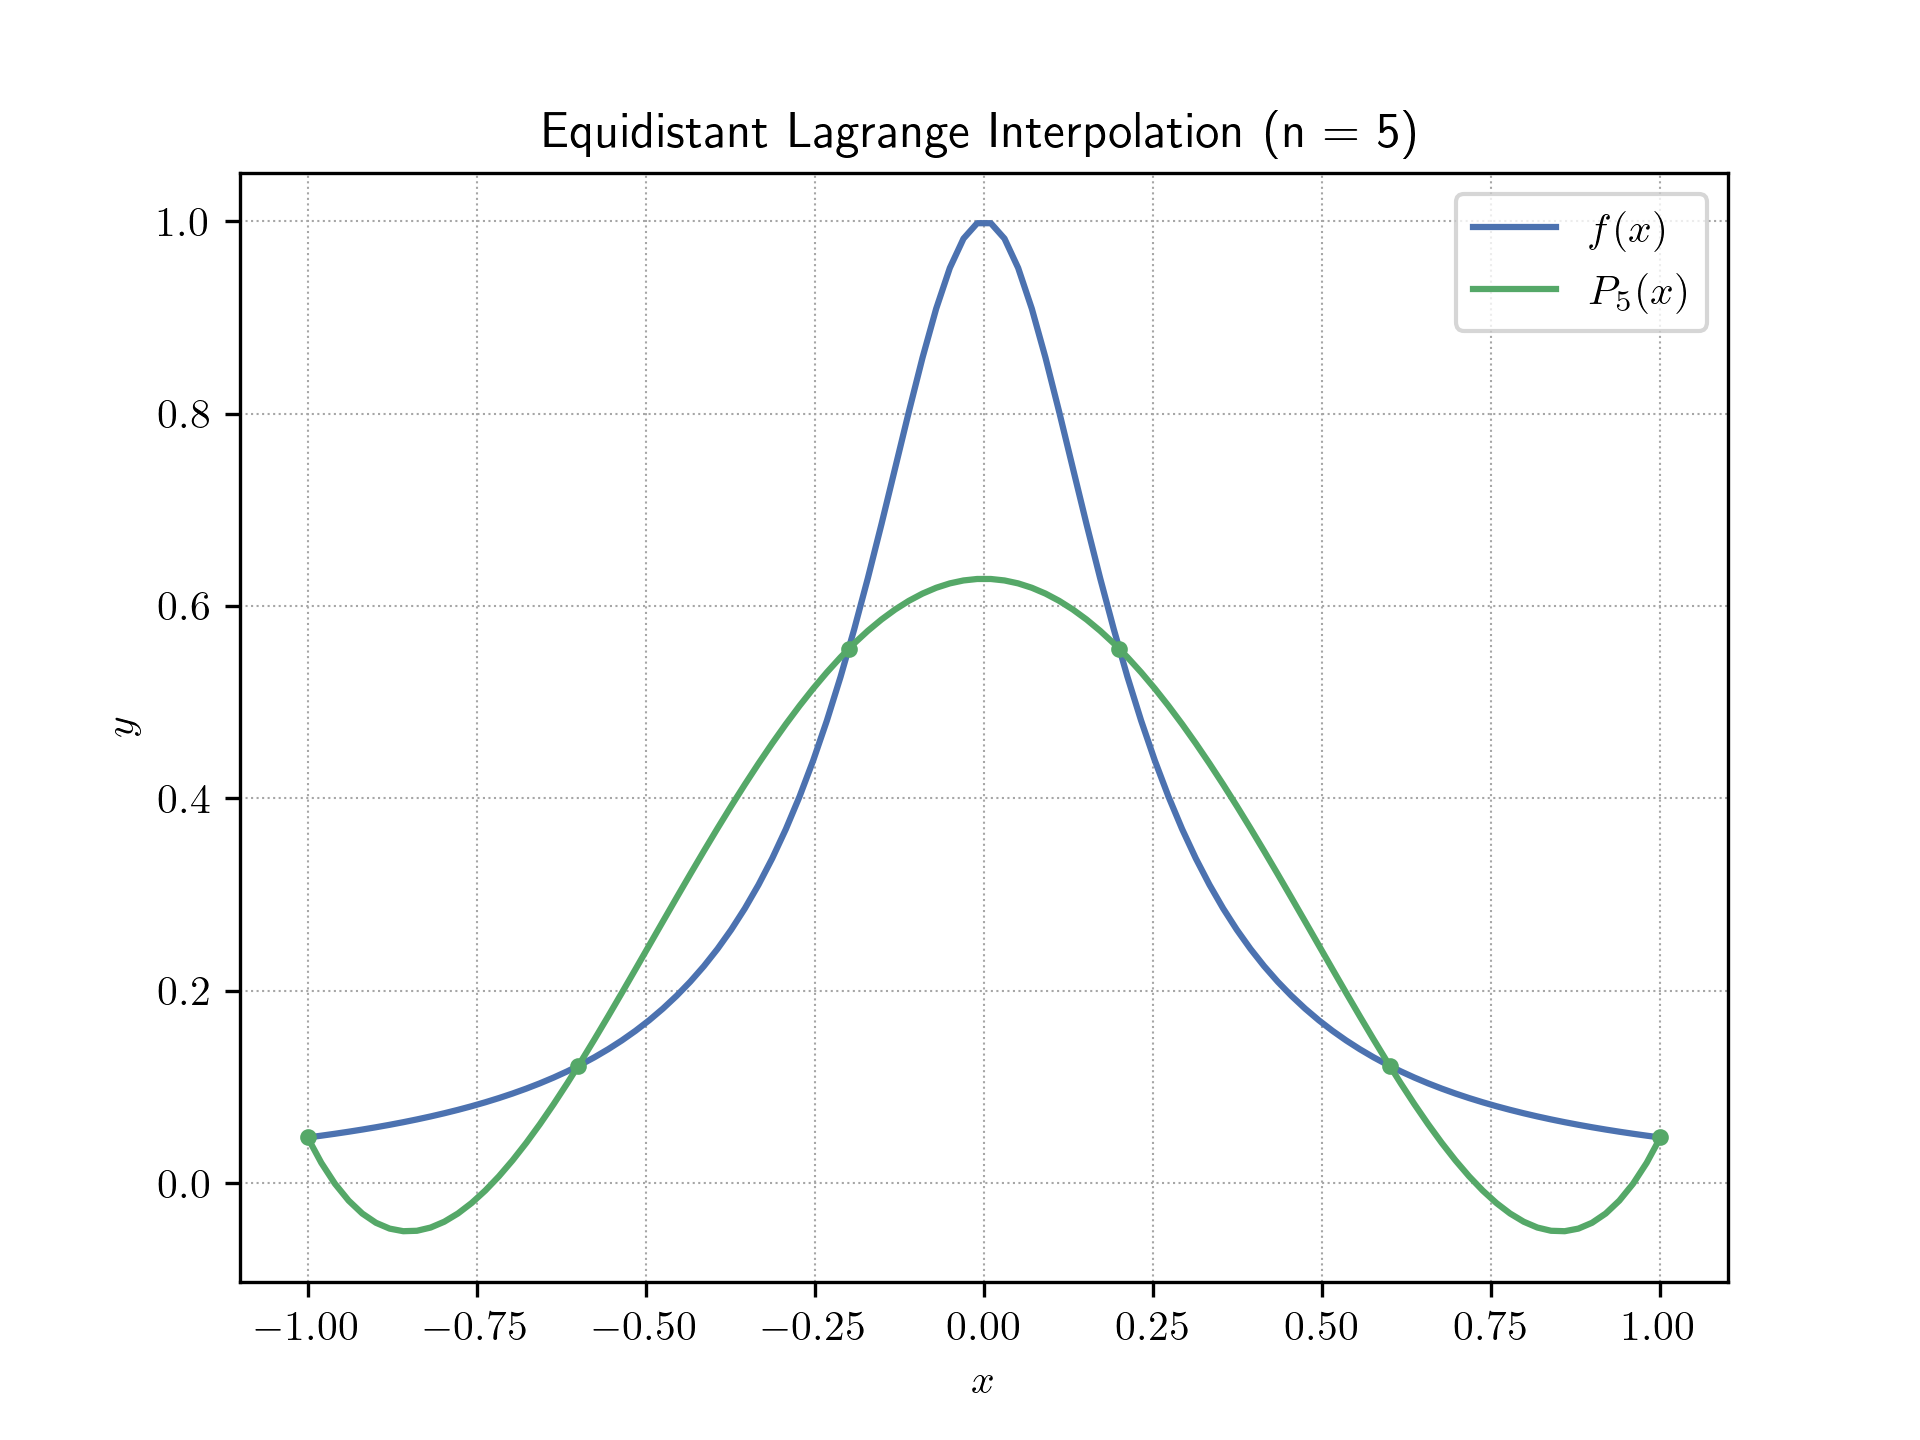
\includegraphics[width=0.8\textwidth]{../plots_2/q2_2/p5.png}
    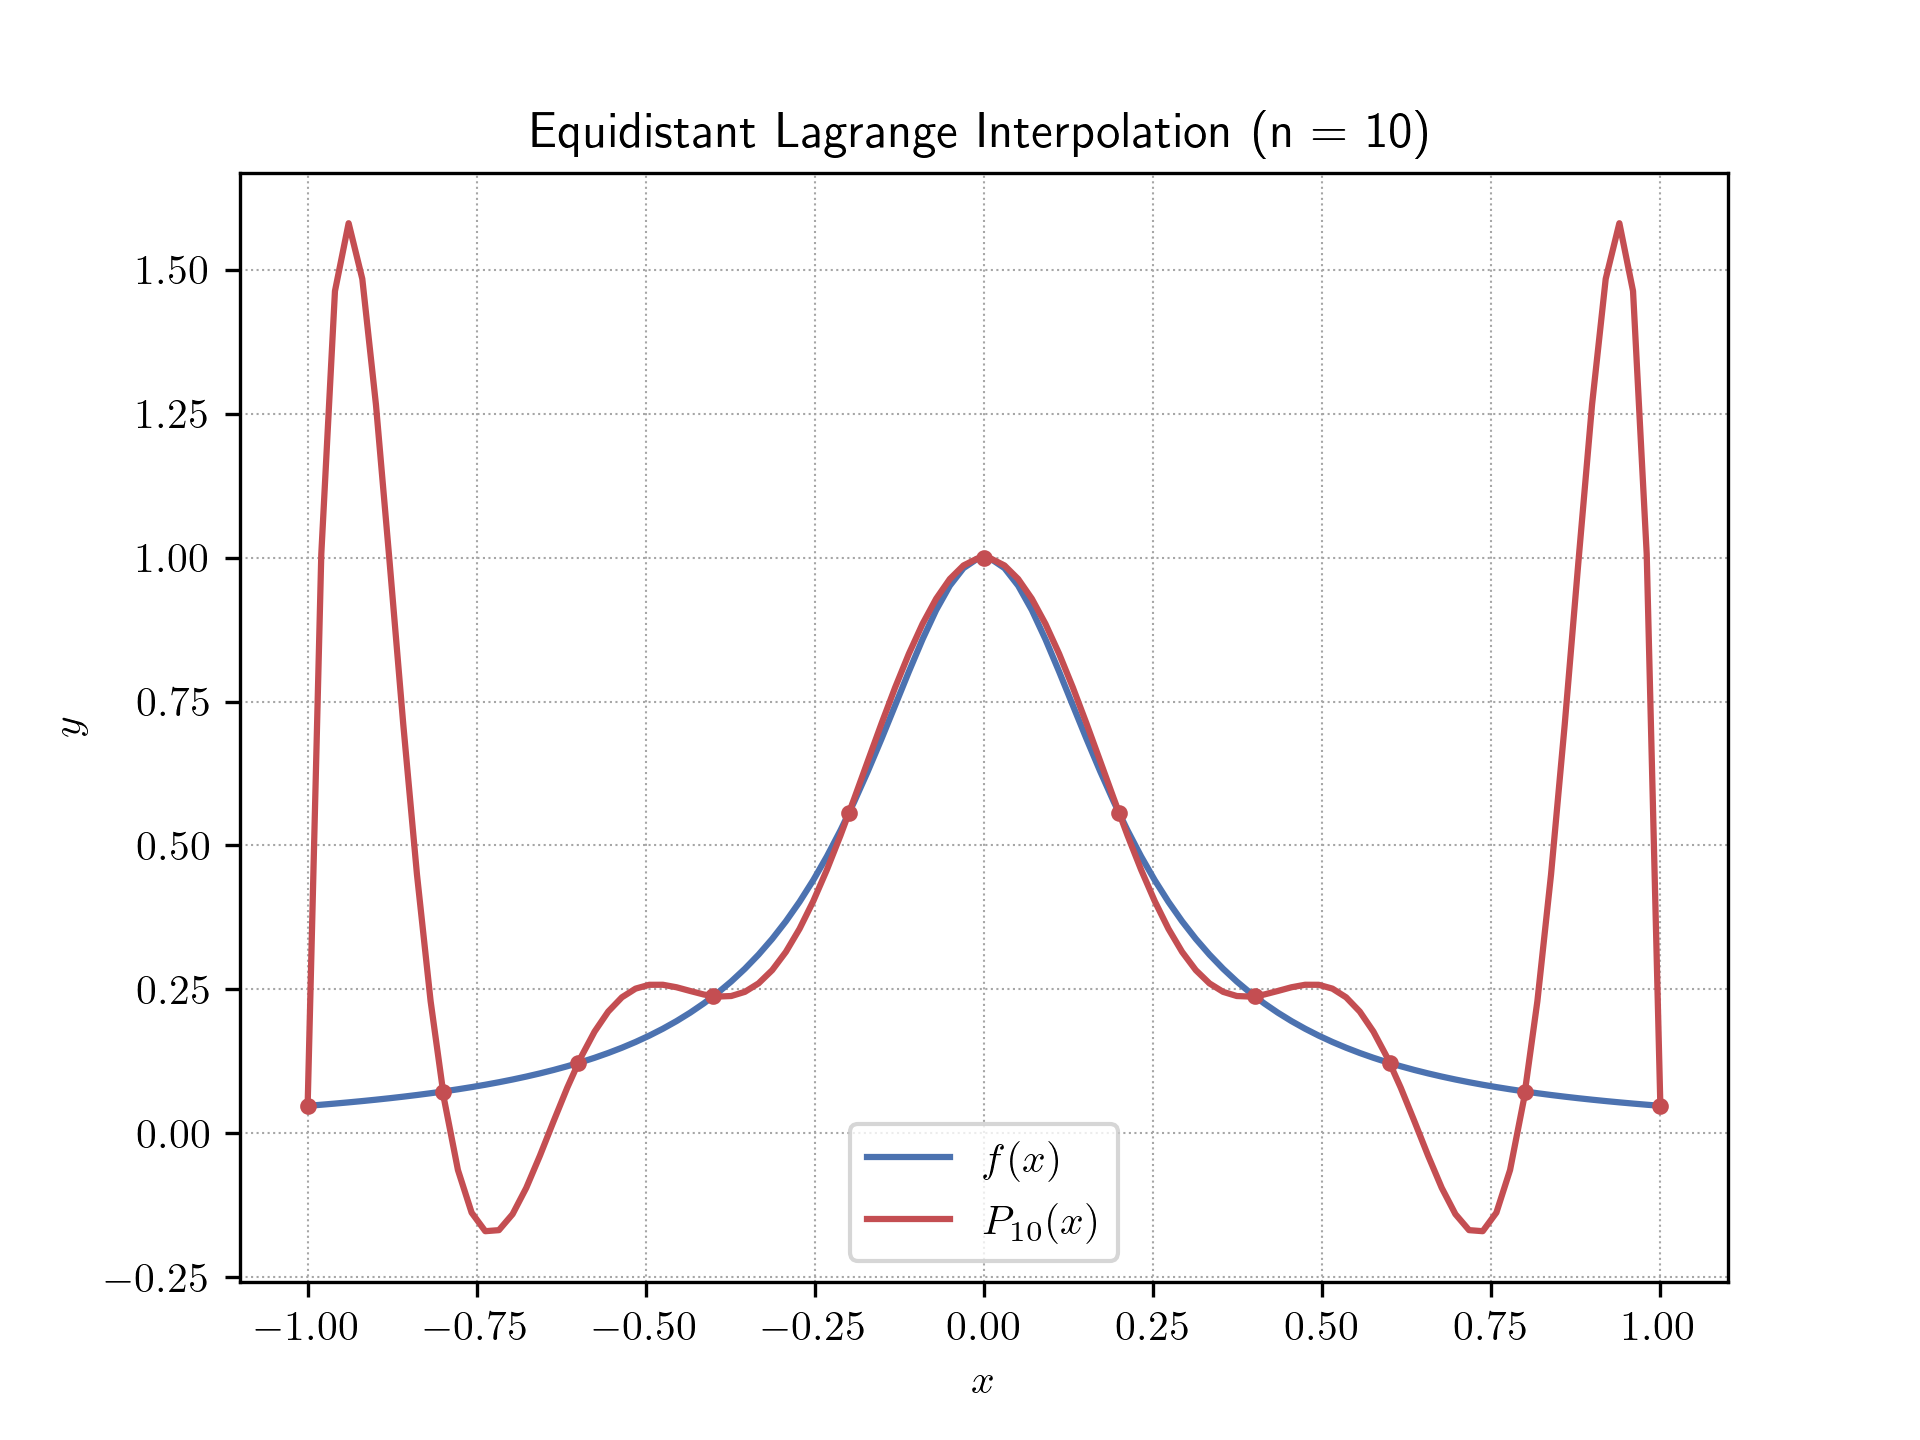
\includegraphics[width=0.8\textwidth]{../plots_2/q2_2/p10.png}
    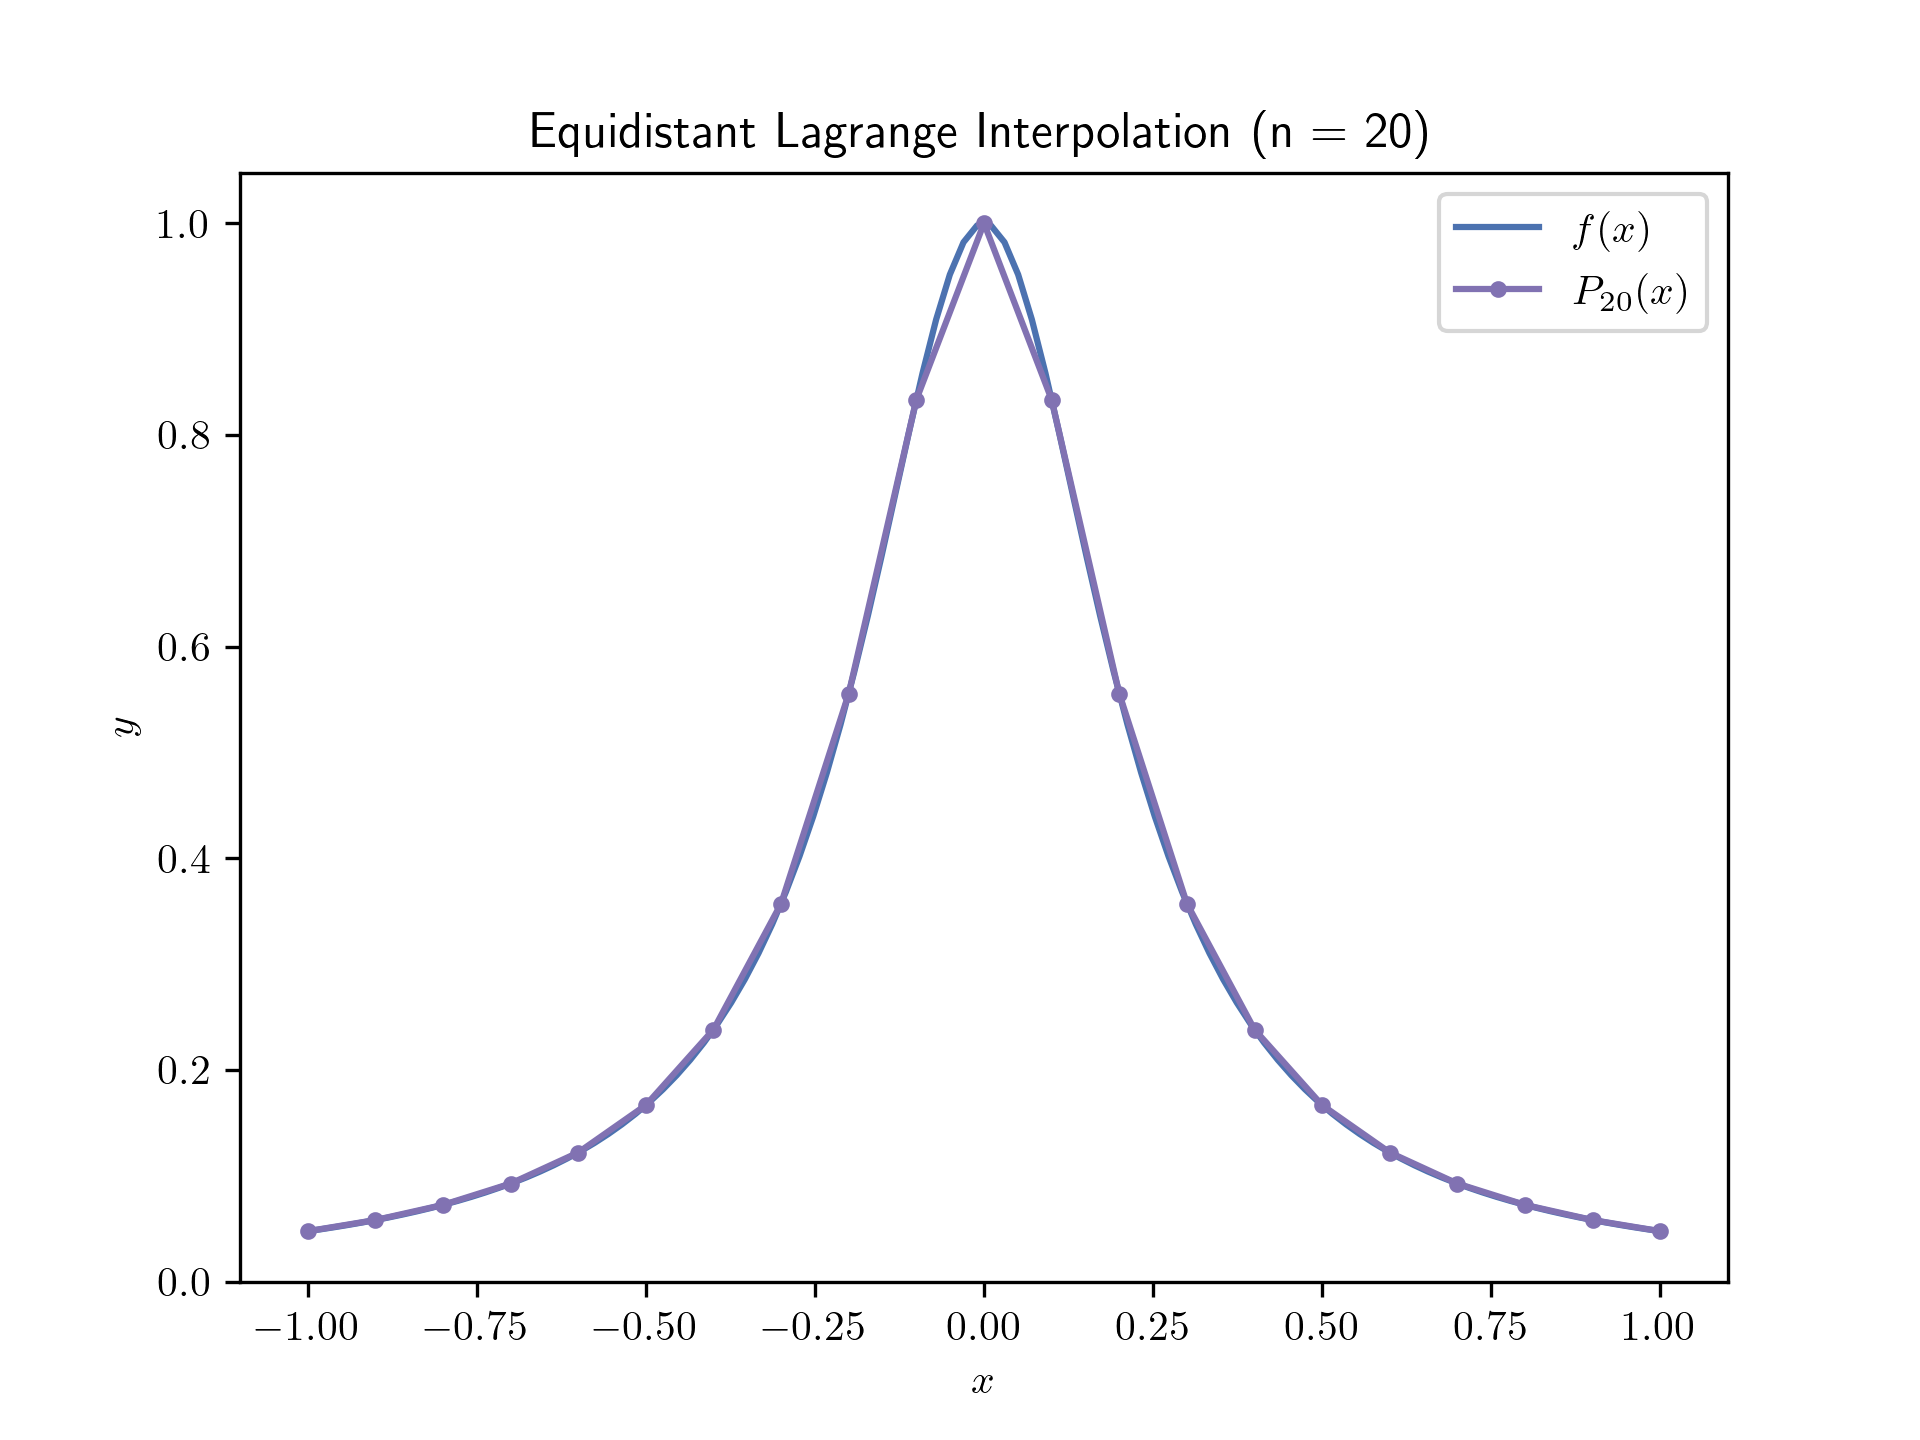
\includegraphics[width=0.8\textwidth]{../plots_2/q2_2/p20.png}
    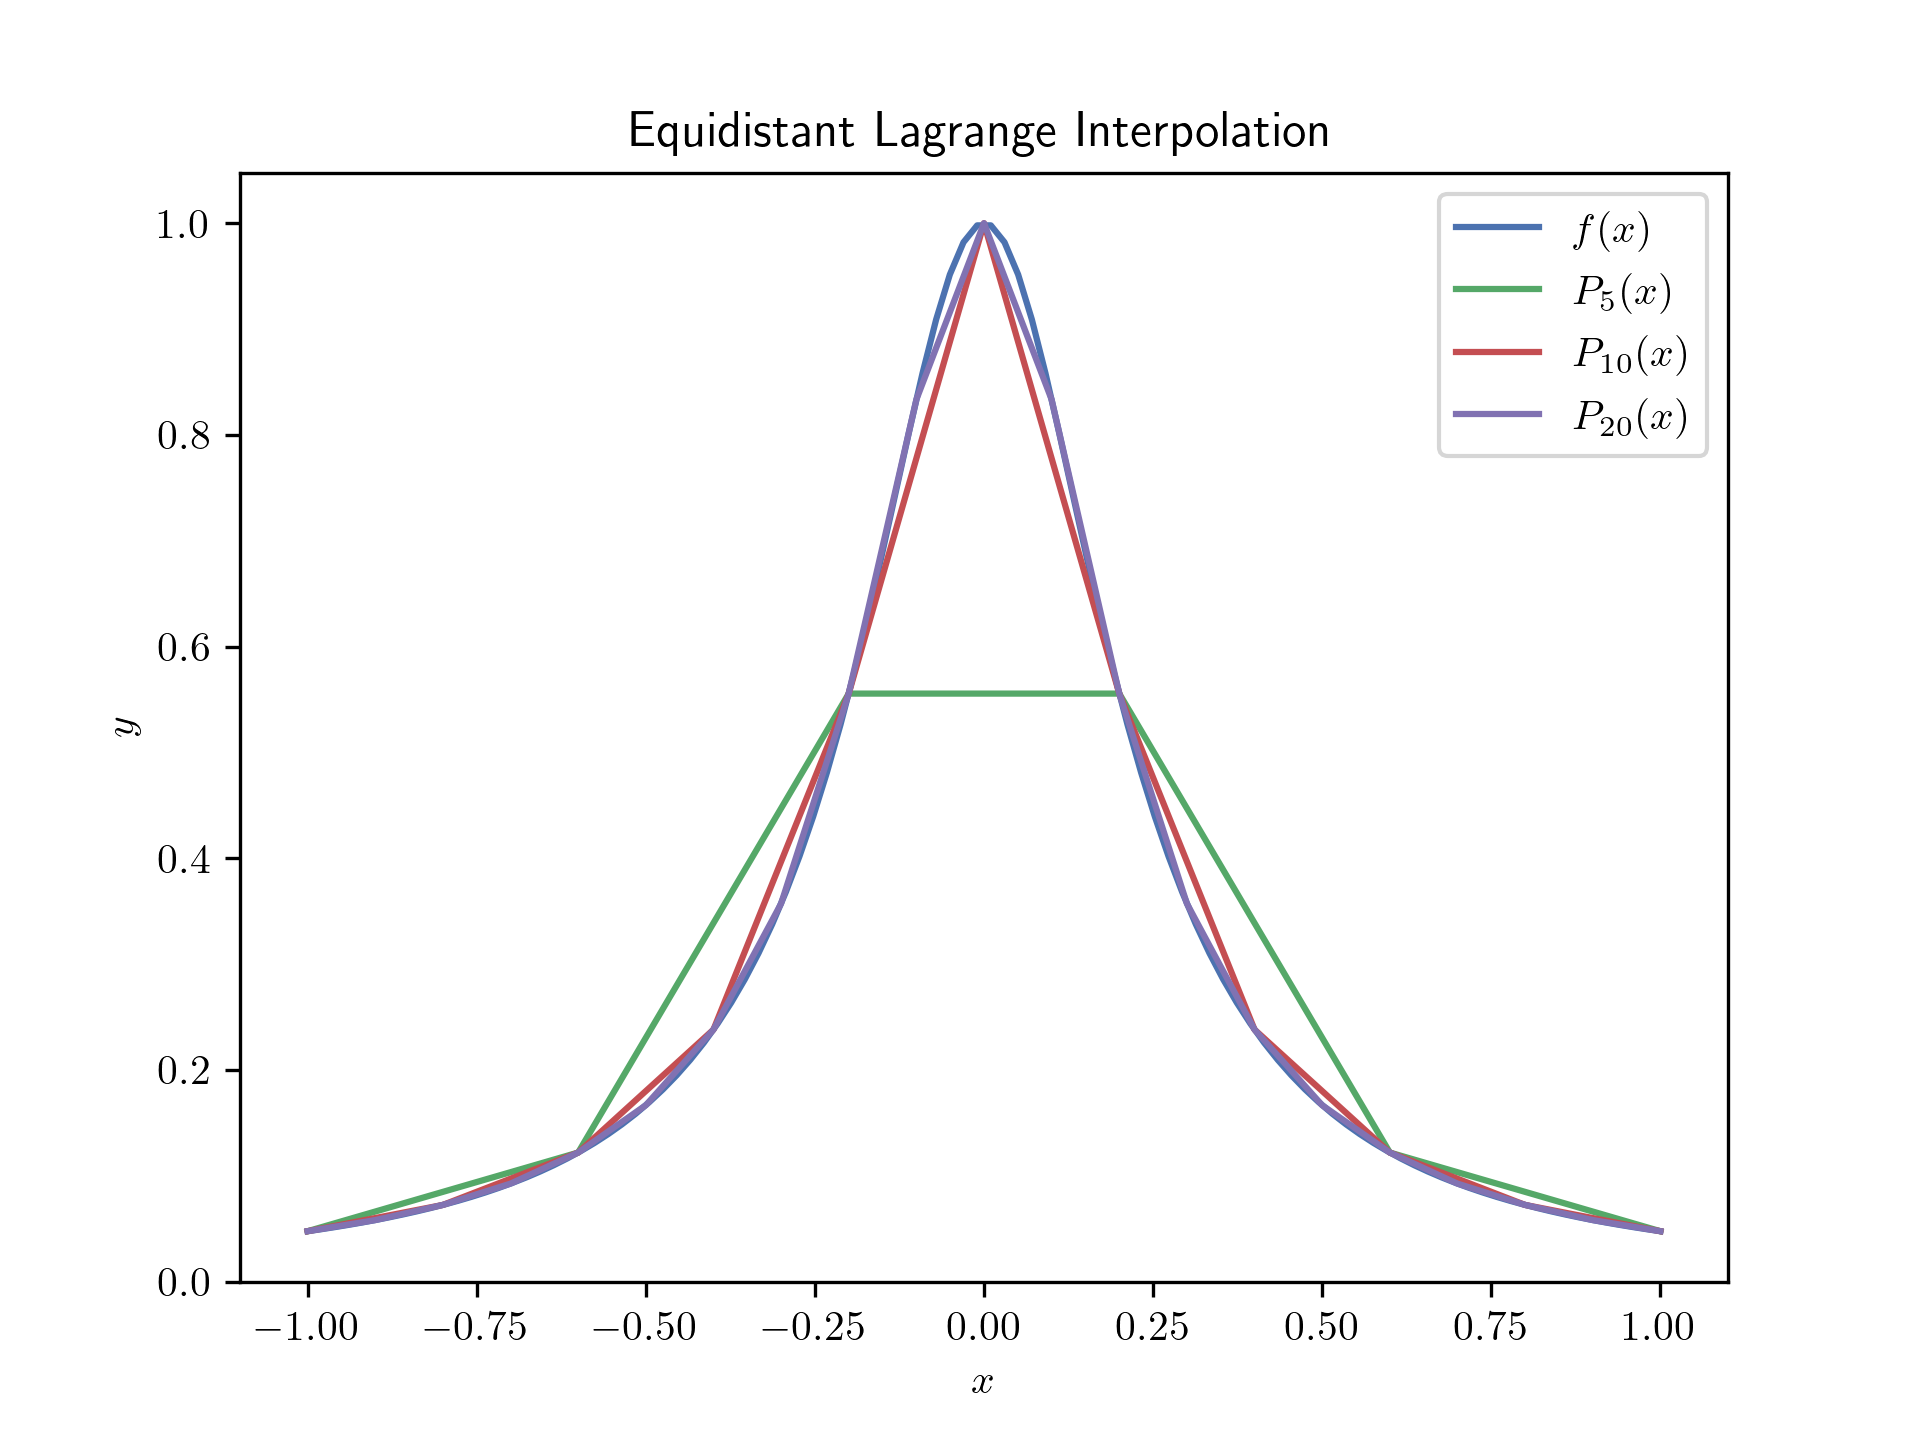
\includegraphics[width=0.8\textwidth]{../plots_2/q2_2/all.png}
\end{center}

As $n$ increases from $5$ to $10$ and $20$, we see that the interpolation error decreases towards the center of the interval $[-1,1]$. However, the error increases significantly near the edges of the interval, demonstrating Runge's phenomenon. 

\newpage
\subquestion
Repeat the interpolation using Chebyshev nodes, and compare the results with the equidistant-node case.

\solution
In addition to the functions defined in the previous parts, the following function was used to generate the Chebyshev nodes:
\begin{lstlisting}[language=Python, caption=2.3 Python]
import numpy as np

def chebyshev_nodes(n):
    nodes = np.array(
        [(math.cos((2 * k - 1) * math.pi / (2 * n))) for k in range(1, n + 1)]
    )

    return nodes
\end{lstlisting}

Th following plots show $f(x)$ and $P_n(x)$ for Chebyshev nodes with $n=5, 10, 20$:
\begin{center}
    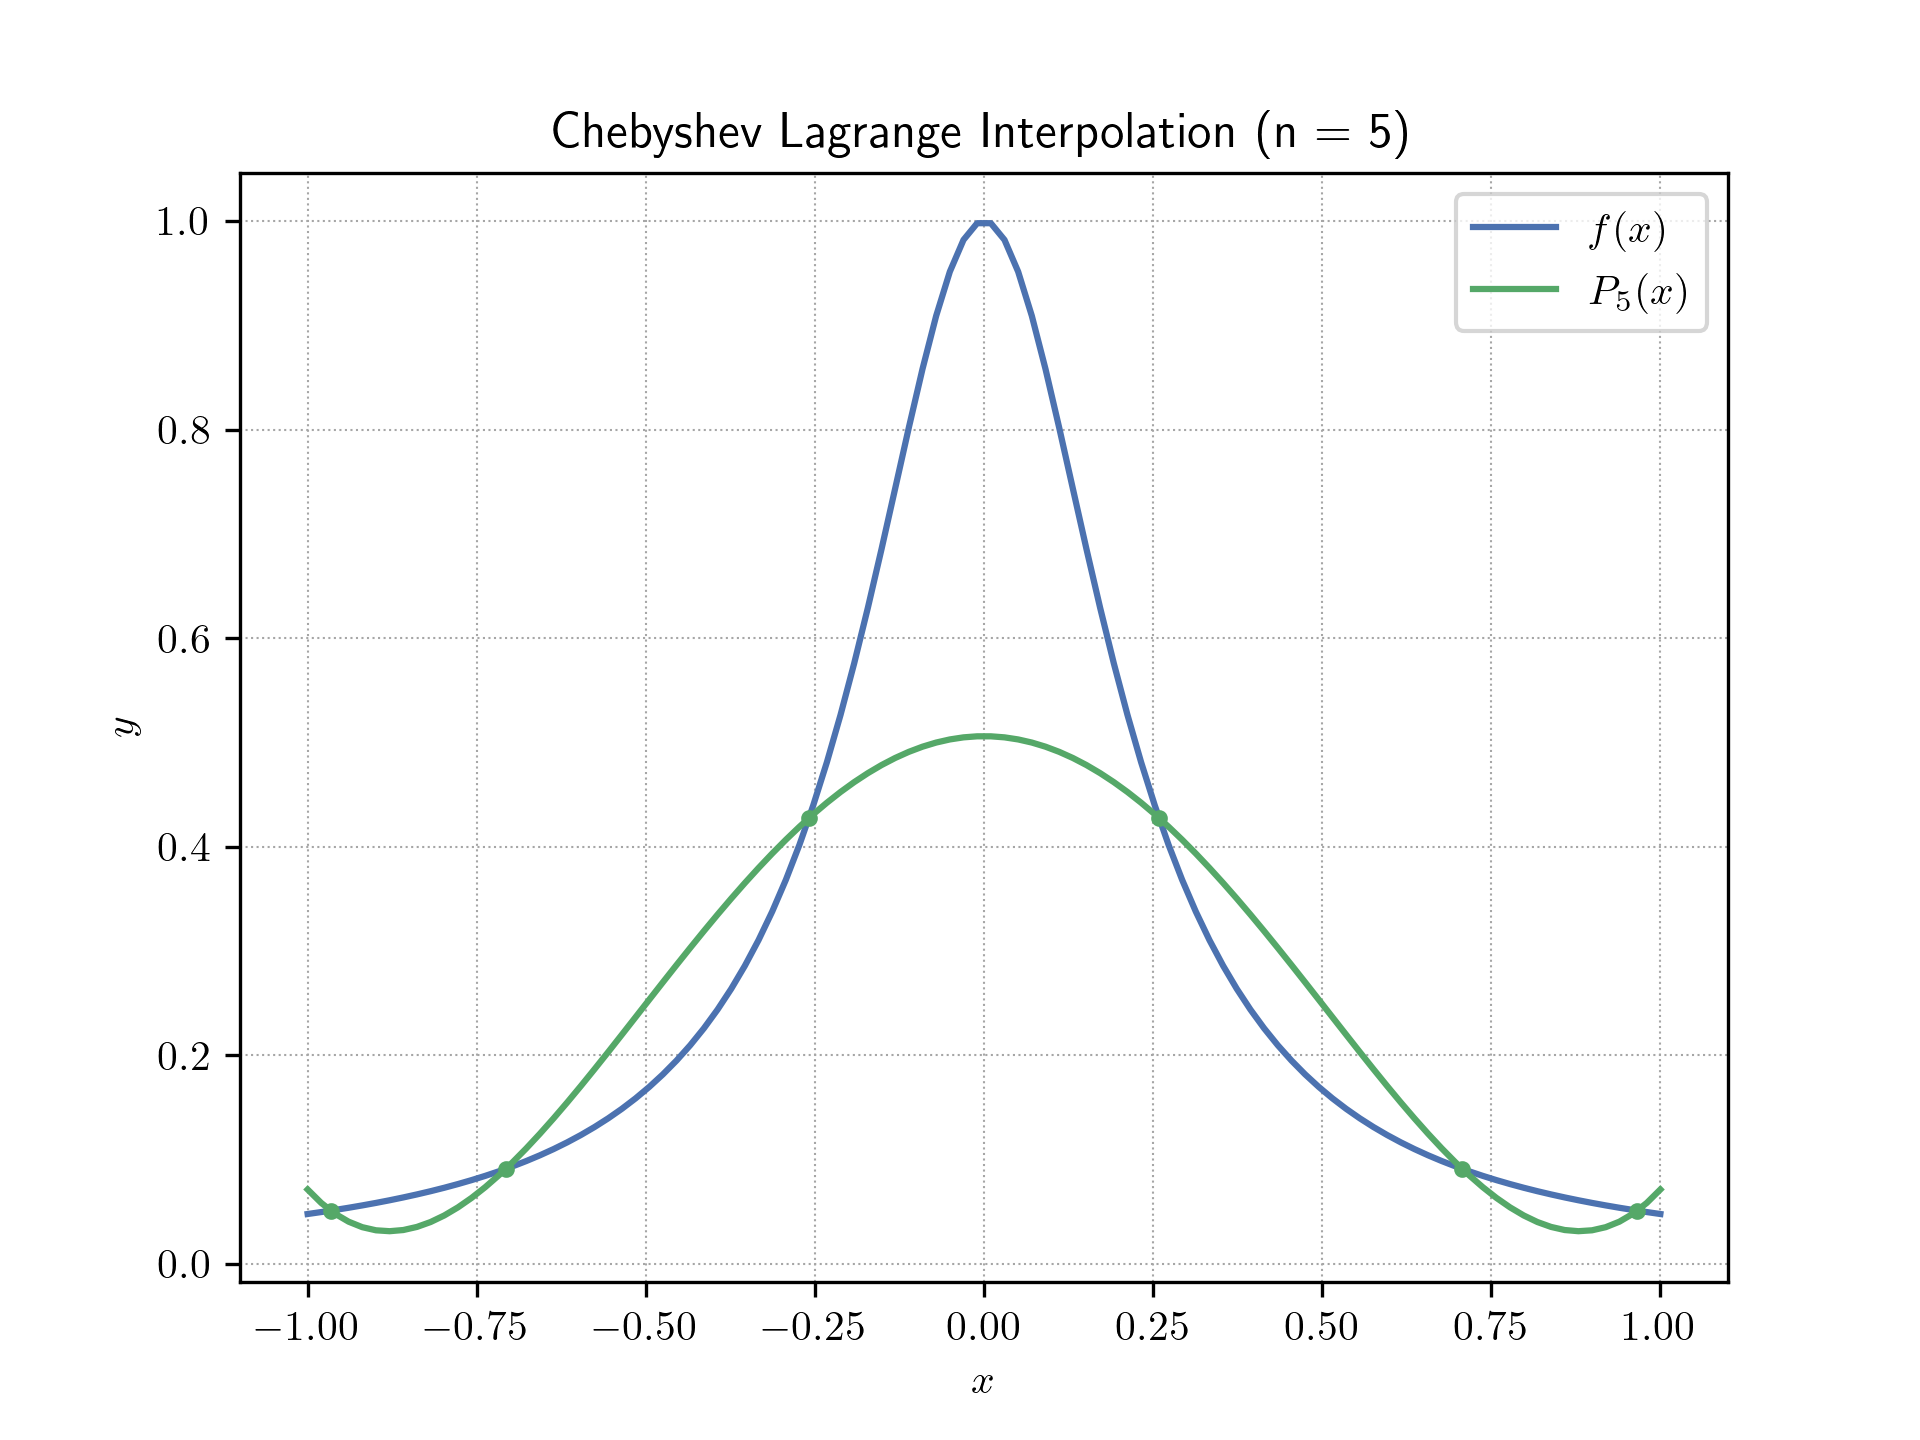
\includegraphics[width=0.8\textwidth]{../plots_2/q2_3/chebyshev_p5.png}
    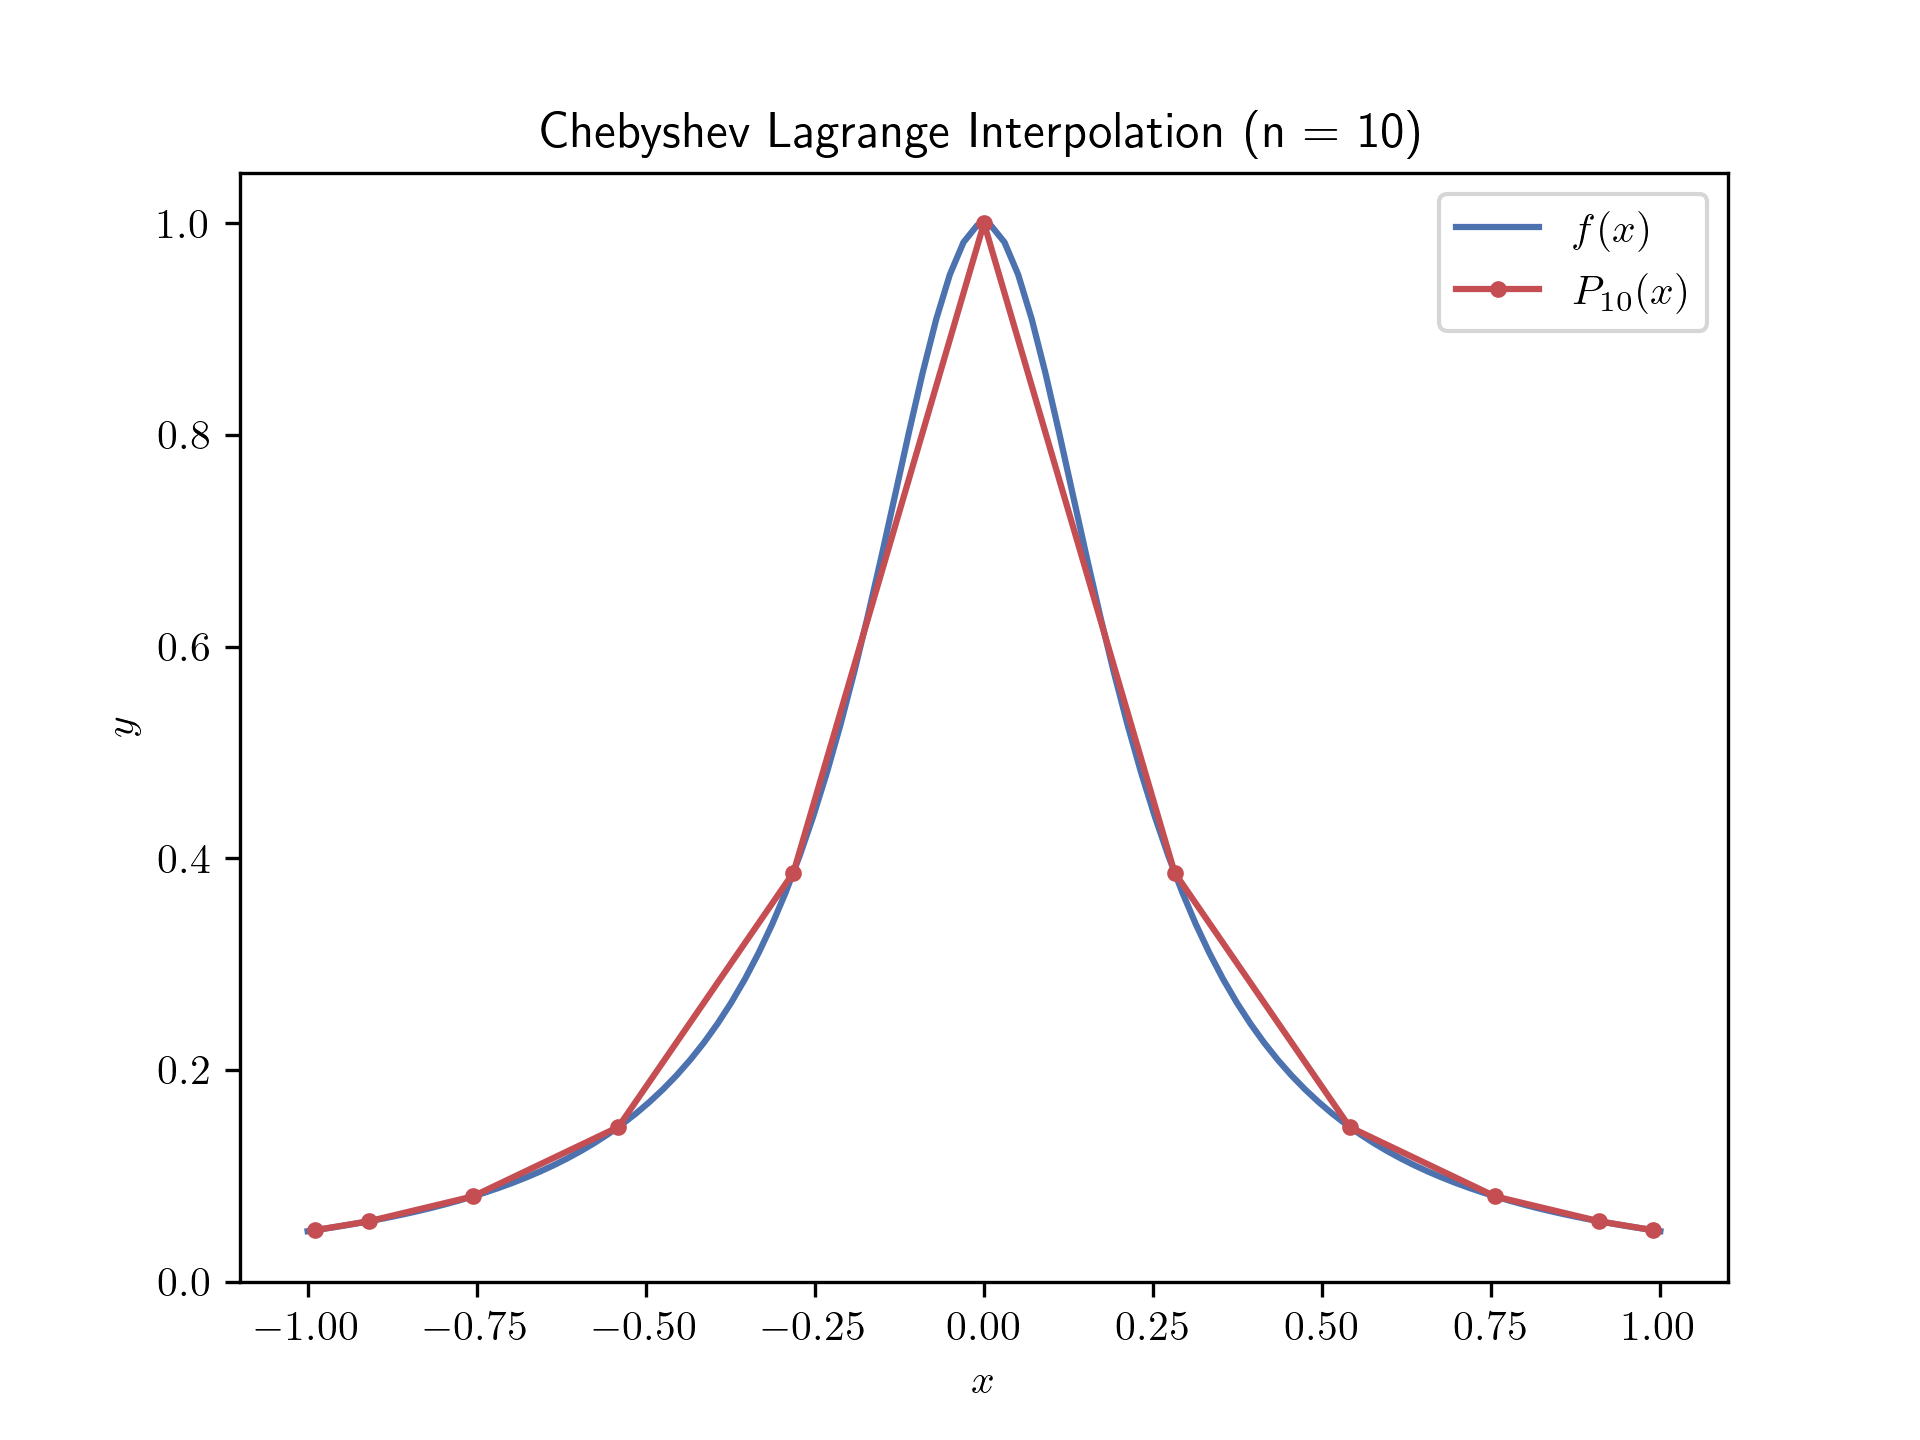
\includegraphics[width=0.8\textwidth]{../plots_2/q2_3/chebyshev_p10.png}
    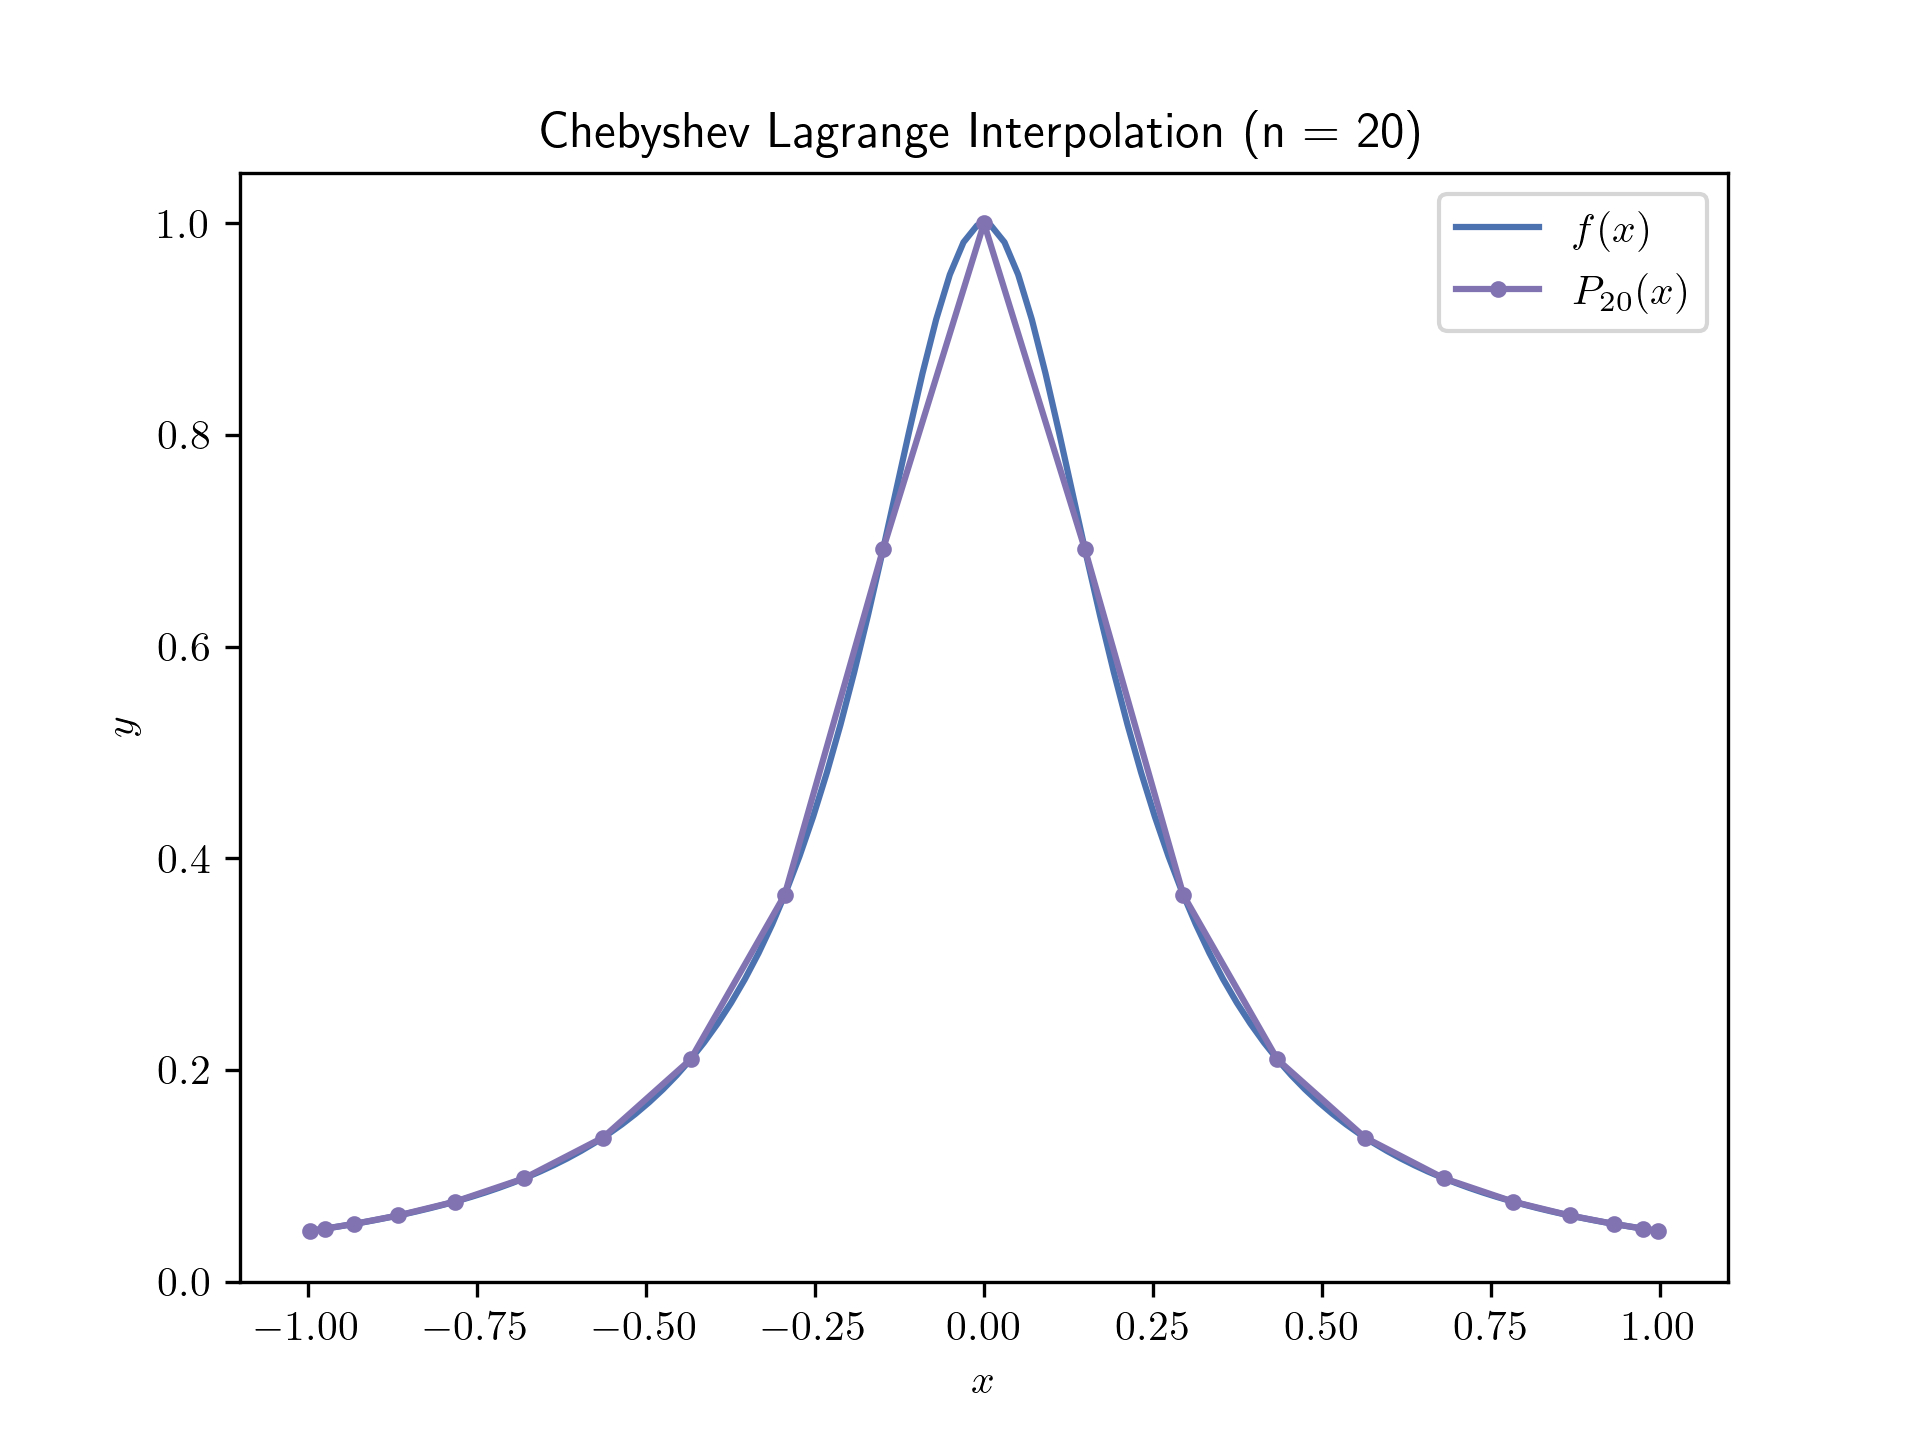
\includegraphics[width=0.8\textwidth]{../plots_2/q2_3/chebyshev_p20.png}
    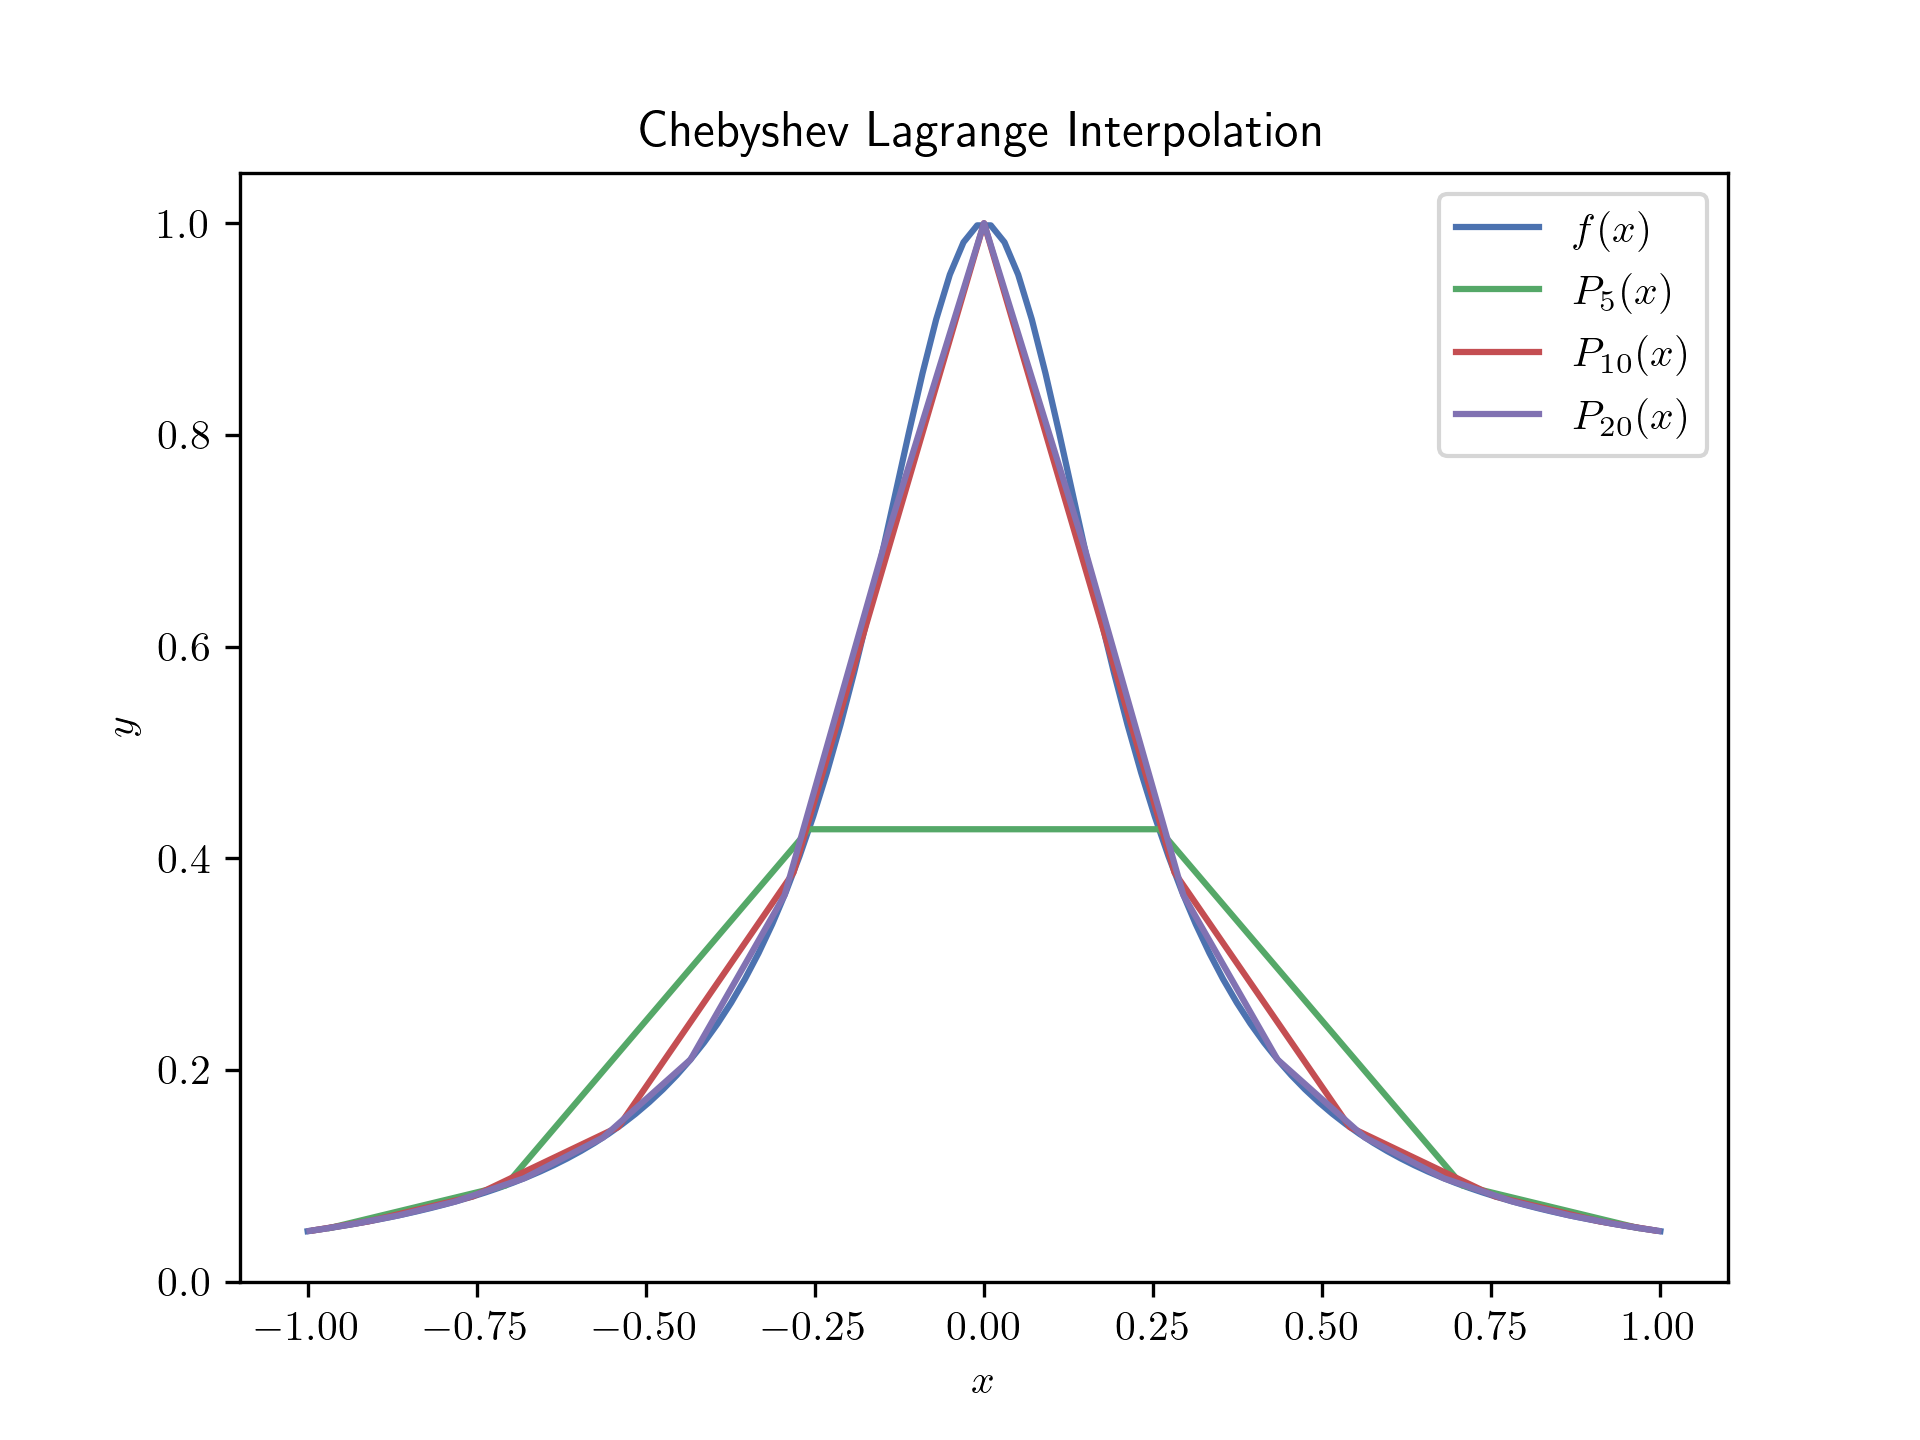
\includegraphics[width=0.8\textwidth]{../plots_2/q2_3/chebyshev_all.png}
\end{center}

Comparing these plots to those with equidistant nodes, we see that using Chebyshev nodes significantly reduces the interpolation error across the entire interval $[-1,1]$. The oscillations near the edges of the interval are much less pronounced, demonstrating that Chebyshev nodes help mitigate Runge's phenomenon and provide a more accurate approximation of $f(x)$.

\newpage
\question{Chebyshev Polynomials and Their Roots}
The Chebyshev polynomials of the first kind is defined by:
\[T_n(x) = \cos(n \arccos x), \quad x \in [-1,1]\]

\subquestion
Prove that the numbers
\[x_k = \cos\left(\frac{2k-1}{2n} \pi\right), \quad k=1,2,\dots,n\]
are the roots of $T_n(x)$.

\subquestion
Show that these roots are distinct and lie in the interval $(-1,1)$.

\subquestion
Write your own code to generate $T_n(x)$ using the recursion formula.

\newpage
\question{Lagrange Interpolation for Nonsmooth Function}
Let $f(x) = |x|$ on the interval $[-1,1]$.

\subquestion
Construct the interpolation polynomial $P_n(x)$ for equidistant nodes when $n$ is even.

\subquestion
Show that $P_n(x)$ is an even polynomial.

\subquestion
Investigate analytically (for small $n$) how well $P_n(x)$ approximates $f(x)$.

\subquestion
Discuss why convergence may be slower for nonsmooth functions.

\end{document}